\chapter{Analytical BER of an AWGN Channel}
\label{appendix:analytical_ber}

Consider an \acf{AWGN} channel as illustrated in figure~\ref{fig:awgn_channel}.

\begin{figure}[htbp]
    \centering
    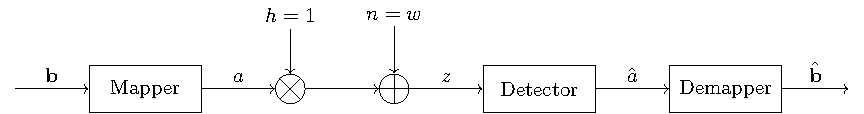
\includegraphics[width=\textwidth]{figures/annex/B_analytical_ber/out/awgn_channel.pdf}
    \caption{Block diagram of an \ac{AWGN} Channel}
    \label{fig:awgn_channel}
\end{figure}

\begin{figure}[htb]
    \centering
    \begin{subfigure}[c]{0.45\textwidth}
        \centering
        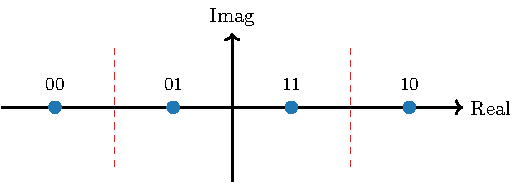
\includegraphics[width=\linewidth]
        {figures/annex/B_analytical_ber/out/4pam_constellation.pdf}
        \caption{4--PAM}
        \label{subfig:4_pam}
    \end{subfigure}
    \vfill
    \vspace{0.65cm}
    \begin{subfigure}[c]{0.475\textwidth}
        \centering
        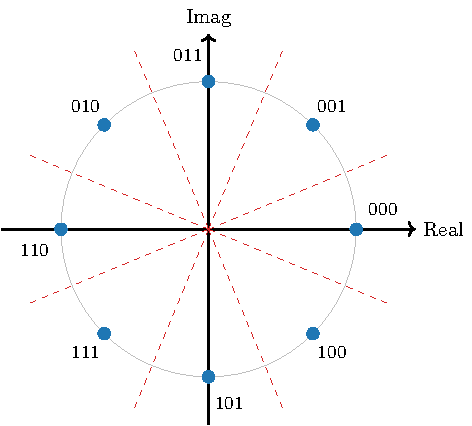
\includegraphics[width=\linewidth]
        {figures/annex/B_analytical_ber/out/8psk_constellation.pdf}
        \caption{8--PSK}
        \label{subfig:8_psk}
    \end{subfigure}
    \hfill
    \begin{subfigure}[c]{0.475\textwidth}
        \centering
        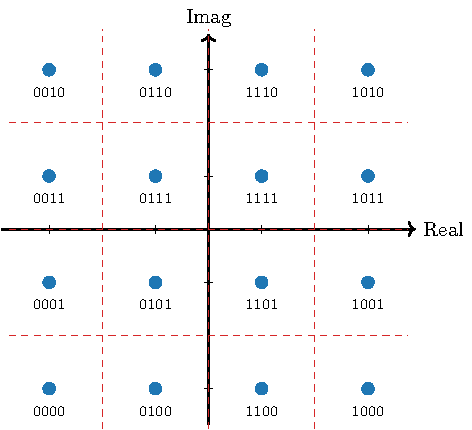
\includegraphics[width=\linewidth]
        {figures/annex/B_analytical_ber/out/16qam_constellation.pdf}
        \caption{16--QAM}
        \label{subfig:16_qam}
    \end{subfigure}
    \caption[Constellation Diagrams]
    {An example of the constellation diagrams for different modulation schemes: 4--PAM, 8--PSK, and 16--QAM. The decision areas are bordered by the red dashed lines.}
    \label{fig:constellations}
\end{figure}


\section{Union Upper Bound}
\label{appendix_section:union_upper_bound}
% =========================
%   Union Upper Bound
% =========================



\section{Nearest Neighbour Approximation}
\label{appendix_section:nn_approximation}
% =======================================
%     Nearest Neighbour Approximation
% =======================================
